\pdfoutput=1
% Options for packages loaded elsewhere
\PassOptionsToPackage{unicode}{hyperref}
\PassOptionsToPackage{hyphens}{url}
\PassOptionsToPackage{dvipsnames,svgnames,x11names}{xcolor}
%
\documentclass[
]{article}
\usepackage{amsmath,amssymb}
\usepackage[T1]{fontenc}
\usepackage[utf8]{inputenc}
\usepackage{textcomp} % provide euro and other symbols
\usepackage{lmodern}
% Use upquote if available, for straight quotes in verbatim environments
\IfFileExists{upquote.sty}{\usepackage{upquote}}{}
\IfFileExists{microtype.sty}{% use microtype if available
  \usepackage[]{microtype}
  \UseMicrotypeSet[protrusion]{basicmath} % disable protrusion for tt fonts
}{}
\makeatletter
\@ifundefined{KOMAClassName}{% if non-KOMA class
  \IfFileExists{parskip.sty}{%
    \usepackage{parskip}
  }{% else
    \setlength{\parindent}{0pt}
    \setlength{\parskip}{6pt plus 2pt minus 1pt}}
}{% if KOMA class
  \KOMAoptions{parskip=half}}
\makeatother
\usepackage{xcolor}
\usepackage{longtable,booktabs,array}
\usepackage{calc} % for calculating minipage widths
% Correct order of tables after \paragraph or \subparagraph
\usepackage{etoolbox}
\makeatletter
\patchcmd\longtable{\par}{\if@noskipsec\mbox{}\fi\par}{}{}
\makeatother
% Allow footnotes in longtable head/foot
\IfFileExists{footnotehyper.sty}{\usepackage{footnotehyper}}{\usepackage{footnote}}
\makesavenoteenv{longtable}
\setlength{\emergencystretch}{3em} % prevent overfull lines
\providecommand{\tightlist}{%
  \setlength{\itemsep}{0pt}\setlength{\parskip}{0pt}}
\setcounter{secnumdepth}{-\maxdimen} % remove section numbering
\usepackage{tikz}
\usetikzlibrary{arrows.meta,positioning}
\setlength{\LTcapwidth}{\linewidth}
\usepackage[margin=1in]{geometry}
\IfFileExists{mathpazo.sty}{\usepackage{mathpazo}\linespread{1.05}}{}
\usepackage{xcolor}
\definecolor{linkblue}{RGB}{0,83,155}
\usepackage[font=small,labelfont=bf,skip=6pt]{caption}
\usepackage{etoolbox}
\AtBeginEnvironment{longtable}{\small}
\clubpenalty=10000
\widowpenalty=10000
\displaywidowpenalty=10000
\usepackage[round,semicolon,numbers]{natbib}
\bibliographystyle{IEEEtran}
\IfFileExists{bookmark.sty}{\usepackage{bookmark}}{\usepackage{hyperref}}
\IfFileExists{xurl.sty}{\usepackage{xurl}}{} % add URL line breaks if available
\urlstyle{same}
\hypersetup{
  pdftitle={beamfeat: beam-search feature construction with false-discovery-rate controlled selection},
  pdfauthor={Olanrewaju M. Daramola},
  colorlinks=true,
  linkcolor={linkblue},
  filecolor={linkblue},
  citecolor={linkblue},
  urlcolor={linkblue},
  pdfcreator={LaTeX via pandoc}}

\title{beamfeat: beam-search feature construction with
false-discovery-rate controlled selection}
\author{Olanrewaju M. Daramola\\[2pt]
{\small ORCID: 0009-0006-3327-2047}\\[1pt]
{\small Independent Researcher}}
\date{28 July 2026}

\begin{document}
\maketitle

\begin{abstract}
\noindent Given a table of measurements, \texttt{beamfeat} searches for short
mathematical formulas, such as \((x_0 / x_2) \cdot x_1\) or
\(\log(a)\log(b)\), that explain a quantity of interest, and then
applies a statistical test to decide which of the candidate formulas
reflect real structure rather than coincidence. The result is a model a
person can read as an equation, together with an explicit statement of
how much statistical confidence it carries. Automated formula search
evaluates thousands of candidates against the same data, so some will
fit by chance; \texttt{beamfeat} controls the expected fraction of such
spurious selections (the false discovery rate, FDR) and reports
honestly, through a fitted flag and visible warnings, whenever that
guarantee cannot be given. It is packaged as scikit-learn
\citep{scikit-learn} estimators over numpy \citep{harris2020} and scipy
\citep{virtanen2020}, passing scikit-learn's own compatibility checks,
with optional dimensional analysis that rejects physically meaningless
expressions (metres plus kilograms) before any numerical work.

\end{abstract}

\hypertarget{introduction}{%
\section{Introduction}\label{introduction}}

Researchers who need interpretable models from tabular data, whether
recovering an empirical law, screening engineered features for a
regression, or auditing which constructed variables genuinely relate to
an outcome, currently choose between tools that construct features
without error control and tools that control errors without constructing
features. The selection step is the scientific crux: candidates are
generated adaptively and tested on the same data, a selective-inference
setting \citep{taylor2015, wasserman2009}: the data that suggested each
hypothesis also tests it, so naive p-values are optimistically biased.
\texttt{beamfeat} treats that step as the inference problem it is. It
provides an exact permutation test of marginal association, each
candidate's relationship to the target considered alone
\citep{phipson2010}, with Benjamini--Hochberg \citep{bh1995} or
Benjamini--Yekutieli \citep{by2001} correction, the knockoff filter in
both its fixed-X \citep{barber2015} and model-X \citep{candes2018}
forms, routed by sample size to the regime where each construction's
assumptions hold, and a default data split (search on one half of the
training rows, selection tested on the other) in the sense of Cox
\citep{cox1975}, which restores the premise the guarantees require: that
candidates were fixed before seeing the data on which they are tested.

\hypertarget{related-work}{%
\section{Related work}\label{related-work}}

\texttt{autofeat} \citep{horn2019} is the closest predecessor: compact
symbolic features feeding a linear model, with exhaustive expansion and
an L1-based selection thresholded against injected noise columns:
effective, but with no stated error-rate guarantee. \texttt{OpenFE}
\citep{zhang2023} generates features for gradient-boosted models and
ranks them by boosting-based importance; Deep Feature Synthesis
\citep{kanter2015} targets relational data; the reference knockoffs
implementation \texttt{knockpy}
\citep{barber2015, candes2018, spector2022} selects among \emph{given}
features and constructs nothing, so its row in the benchmark table below
isolates the contribution of construction itself. Symbolic regressors
such as \texttt{PySR} \citep{cranmer2023} conduct a strictly more
powerful expression search, fitting constants inside nonlinearities,
with no error control. The closest design precedent is \texttt{tsfresh}
\citep{christ2018}, which filters mass-generated time-series features
under Benjamini--Yekutieli control; \texttt{beamfeat} brings that
generate-then-error-controlled-filter design to symbolic expressions on
tabular columns.

Contributing the guarantee to an existing tool was not viable: it
requires a different selection statistic (exact under permutation), a
holdout architecture threaded through the fit path, and an expression
engine whose numerical failures are recorded rather than masked: a
redesign of each tool's core rather than a patch. The practical case is
also material: during benchmarking, neither \texttt{autofeat} 2.1.3 nor
\texttt{OpenFE} 0.0.12 ran on a current stack without intervention.
\texttt{autofeat} raises
\texttt{TypeError:\ check\_array()\ got\ an\ unexpected\ keyword\ argument\ \textquotesingle{}force\_all\_finite\textquotesingle{}}
whenever it transforms or predicts on unseen data having engineered at
least one feature, on scikit-learn \(\geq\) 1.8 (the argument was
renamed in 1.6 and removed in 1.8), that is, in its normal supervised
use, and its pins (\texttt{numpy\textless{}2.0},
\texttt{pandas\textless{}3.0}) downgrade current environments.
\texttt{OpenFE} calls \texttt{mean\_squared\_error} with the
\texttt{squared} argument removed in scikit-learn 1.6. Both were
therefore run in isolated environments, with the \texttt{OpenFE}
compatibility patch disclosed in the repository's benchmark code, while
\texttt{beamfeat}'s tests run unmodified from scikit-learn 1.6 through
1.9 with no upper version pins.

\hypertarget{method}{%
\section{Method}\label{method}}

Three trade-offs define the design. First, the selection statistic is
\emph{marginal} association, absolute Pearson correlation for regression
and eta-squared (the correlation ratio for class labels) for
classification: a fixed function of the data, so permutation p-values
are exact, where statistics that re-tune themselves on the observed
target (a cross-validated lasso penalty) break the exchangeability a
permutation test rests on (under the null, the target and its shuffles
are statistically interchangeable; a statistic that adapts to the
observed target destroys that symmetry). The price is measured precisely
on Friedman \#1 \citep{friedman1991}. A least-squares oracle given the
ideal depth-2 basis \(\{ab, (ab)^2, c, c^2, d, e\}\) reaches \(R^2\)
\(0.960 \pm 0.003\) over six draws. Marginal screening never admits
\(c\), because the centred quadratic viewed alone is nearly independent
of the target; it admits \(c^2\) on some draws and not others, since
\((c-0.5)^2\) expands to carry a little marginal signal through that
term. The best any model restricted to the admitted set can reach is
\(0.874 \pm 0.006\), against the pipeline's \(0.776 \pm 0.013\). Roughly
0.086 is lost to what marginal screening cannot see and 0.098 to the
search. Part of that remaining gap is a search limitation that persisted
under wider beams, greater candidate diversity, and lookahead scoring;
closing it fully would require scoring candidates as a set rather than
one at a time, which reintroduces exactly the pick-what-fits-the-noise
behaviour the design excludes. Heuristic tools that select jointly
outperform on this structure while certifying nothing.

\begin{figure}[tbp]
\centering
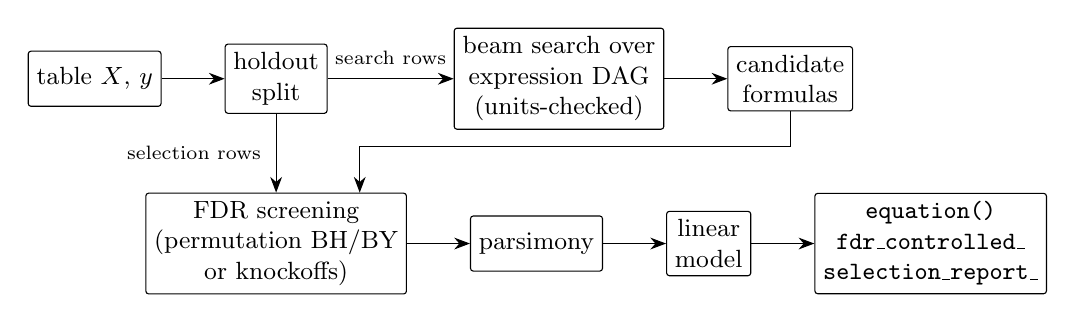
\begin{tikzpicture}[
  node distance=4mm and 8mm, >={Stealth[length=2mm]},
  box/.style={draw, rounded corners=1pt, align=center, font=\small,
              inner sep=3pt, minimum height=7mm},
  lab/.style={font=\scriptsize}
]
\node[box] (xy) {table $X$, $y$};
\node[box, right=of xy] (split) {holdout\\split};
\node[box, right=16mm of split] (search) {beam search over\\expression DAG\\(units-checked)};
\node[box, right=of search] (cand) {candidate\\formulas};
\node[box, below=10mm of split] (screen) {FDR screening\\(permutation BH/BY\\or knockoffs)};
\node[box, right=of screen] (pars) {parsimony};
\node[box, right=of pars] (fit) {linear\\model};
\node[box, right=of fit] (out) {\texttt{equation()}\\\texttt{fdr\_controlled\_}\\\texttt{selection\_report\_}};
\draw[->] (xy) -- (split);
\draw[->] (split) -- node[lab, above=0.6mm, pos=0.5]{search rows} (search);
\draw[->] (search) -- (cand);
\draw[->] (cand.south) -- ++(0,-4.5mm) -| ([xshift=-6mm]screen.north east);
\draw[->] (split) -- node[lab, left=0.7mm]{selection rows} (screen);
\draw[->] (screen) -- (pars);
\draw[->] (pars) -- (fit);
\draw[->] (fit) -- (out);
\end{tikzpicture}
\caption{The pipeline: candidates are constructed on one part of the data
and tested on the other, so adaptive search cannot bias the selection
p-values; only screened survivors reach the fitted model.}
\end{figure}

Second, correctness defaults are chosen over power and convenience.
Benjamini--Yekutieli is the estimator default because it is valid under
arbitrary dependence, which is the regime engineered candidates occupy:
they share parents and are mutually correlated by construction, so the
positive dependence Benjamini--Hochberg assumes cannot be taken for
granted. Over 100 pure-noise pipelines, where every selection is by
definition false, BH returned features in 6 trials and BY in 1 (false
discovery proportions 0.06 and 0.01). Both sit under the nominal 0.10
and the difference is not significant at this trial count
(\(p = 0.12\)), but BH fires on noise several times as often, and it is
the tail behaviour a default should be chosen for. When nothing passes
selection, the default returns \emph{no} constructed features (an
intercept-only model and a visible warning) rather than unvetted search
output. A parsimony step (greedy forward selection \emph{within} the
screened set) keeps fitted equations compact while the full screened
set, with exact p- and q-values \citep{storey2002} per candidate, stays
auditable; the q-level guarantee certifies the screening set, and the
documentation says so. A post-fit check on the selection holdout
separates two claims users conflate: FDR-vetted association and a
generalising fit: a negative held-out \(R^2\) raises a visible warning
naming the gap.

Third, boundaries are stated with measurements. Piecewise targets belong
to trees (LightGBM 0.998 against 0.808 on a threshold problem;
\texttt{OpenFE} records 0.998 there as well, but bit-identically to raw
LightGBM and from a feature touching only an irrelevant column, so the
credit belongs to its gradient-boosted consumer rather than to anything
it constructed); the exponential operator ships but is not a default
(enabling it changed no outcome on the physics panel below, though
individual scores move); overflow and domain errors exclude a candidate
loudly rather than silently; and units, supplied as pint quantities or
plain strings, are enforced at expression construction.

\hypertarget{results}{%
\section{Results}\label{results}}

The repository's significance rests on evidence that ships with the code
and can be re-run, rather than on claims. End to end at nominal FDR
0.10, 200 repeated trials with a true signal produced no false discovery
at all, a 95\% upper bound of 0.015 on the true rate, with power 1.000
and no fit falling back to unvetted output; 60 trials with no signal
selected nothing. At the selector level, realised FDR tracked the bound
each correction must respect. Over 100 trials Benjamini--Hochberg
realised \(0.046 \pm 0.008\), \(0.084 \pm 0.012\) and
\(0.161 \pm 0.016\) at nominal 0.05/0.10/0.20, against its ceiling of
\(q\,m_0/m\) = 0.040/0.080/0.160; Benjamini--Yekutieli, stricter by a
harmonic factor, realised \(0.008 \pm 0.004\), \(0.018 \pm 0.005\) and
\(0.046 \pm 0.008\). Power was 1.00 throughout. The bounds are derived
from the design rather than asserted, and
\texttt{benchmarks/selector\_calibration.py} fails if a realised rate
sits \emph{significantly} above its bound, that is, if the bound falls
below the whole 95\% interval; a point estimate a little above its
bound, as all three Benjamini--Hochberg rates are here, is ordinary
Monte Carlo error.

\begin{figure}[tbp]
\centering
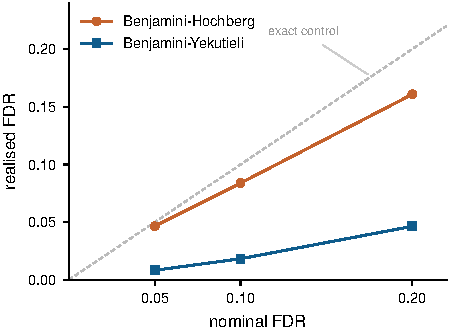
\includegraphics[width=0.62\linewidth]{figures/fig_fdr_calibration.pdf}
\caption{Realised against nominal false discovery rate for the permutation
selector, 100 trials on Gaussian designs with 25 candidates of which 5 carry
signal. Benjamini--Hochberg tracks its ceiling of $q\,m_0/m$; Benjamini--Yekutieli,
stricter by a harmonic factor, sits well below nominal. Power was 1.00 at every
level. Regenerated by \texttt{benchmarks/selector\_calibration.py}, which derives
each bound from the design and fails if the bound falls below a realised rate's 95\% interval.}
\end{figure}

On a twelve-equation physics panel under the symbolic-regression
community's criterion (\(R^2 > 0.999\) at 0.1\% noise)
\citep{lacava2021, udrescu2020}, \texttt{beamfeat} solves 10/12 and
recovers 8/12 in \emph{exact symbolic form}, checked by algebraic
proportionality, a test a merely close numeric fit cannot pass, at
roughly 0.6 s per equation; each miss marks a named boundary (a depth-3
rational, a literal constant, a depth-4 nesting, the Gaussian's
exponential).

Head-to-head, using the benchmark code shipped in the repository
(identical data splits; each compared tool run in an environment
matching its own declared dependencies):

\begin{table}[tbp]
\centering
\small
\caption{Benchmark results from the repository's benchmark code.
\texttt{OpenFE}'s recovery figure is over five of the six stress datasets; its
core-suite rows are not applicable, since it targets gradient-boosted lift
rather than formulas. It ran only on the stress suite: its recovery and
false-feature entries cover the five stress problems that declare generating
columns, and its fit time averages all six, so that cell is not directly
comparable to the core-suite times in the other columns.}
\label{tab:headtohead}
\begin{tabular}{@{}lrrrrrr@{}}
\toprule
measure & beamfeat & autofeat & OpenFE & knockpy & LightGBM & ridge \\
\midrule
generating columns recovered & \textbf{10/10} & 8/10 & 0/5 & 0/10 & --- & --- \\
mean $R^2$, core suite & \textbf{0.9989} & 0.9968 & --- & 0.8450 & 0.9798 & 0.8442 \\
stress sets with false features & \textbf{0 of 5} & 3 of 5 & 0 of 5 & 1 of 5 & --- & --- \\
mean fit time (s) & \textbf{0.2} & 12 & 1.4 & 0.02 & 0.3 & $<$0.01 \\
\bottomrule
\end{tabular}
\end{table}

Two ten-problem sets underlie Table~\ref{tab:headtohead} and they are not the
same ten. Recovery asks whether some returned feature references all of the
generating columns, over the ten synthetic problems that declare them; the mean
$R^2$ column covers the ten formula-recovery problems of the core suite, which
substitutes \texttt{purely\_linear} for \texttt{heavy\_tail\_t2}. Fit times are
indicative figures from one machine (Dell Inspiron 16 Plus 7640, 22 logical
cores, Linux 7.0, Python 3.11.15, scikit-learn 1.7.2, numpy 1.26.4, no
accelerator), the pinned environment the compared tools require; the
cross-method ratios, measured on identical hardware, are the stable quantity.

Under Student-\(t(2)\) noise the exact formula is recovered at \(R^2\)
0.956 (LightGBM 0.866): the permutation test is distribution-free (it
assumes nothing about the noise's shape). Across seven real datasets
\citep{gorman2014}, \texttt{beamfeat} leads on two: mpg (0.871 against
LightGBM's 0.853) and tips, where gradient boosting overfits below ridge
while the FDR gate holds; it matches ridge on diamonds from a single
interpretable feature, and trails LightGBM on penguins and breast cancer
and ridge on diabetes. The widest margin against it is California
housing, at 0.700 against LightGBM's 0.843, where the signal is spatial
rather than algebraic and there is no compact expression to find; it
still clears the ridge anchor there by 0.107. A feature constructor
should concede when there is nothing to construct, and the honesty flag
does so on every fit.

\begin{figure}[tbp]
\centering
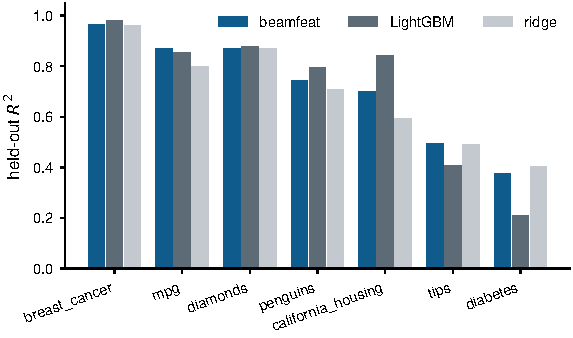
\includegraphics[width=0.85\linewidth]{figures/fig_real_datasets.pdf}
\caption{Held-out $R^2$ on seven real datasets, numeric columns only.
\texttt{beamfeat} leads on mpg and tips, matches ridge on diamonds from a
single constructed feature, and trails the gradient-boosted baseline where the
signal is not algebraic. California housing is the widest margin against it:
the structure there is spatial, and there is no compact expression to find.}
\end{figure}
 A separate 360-fit study, included in the
repository (nine datasets \citep{yeh1998, cortez2009, harrison1978},
eight methods, five splits, analysed by average ranks and a Friedman
test \citep{demsar2006}) places these results in a wider field. One of
the nine is the Boston housing set, which scikit-learn removed as
ethically contested; it is retained here deliberately, because the
\texttt{autofeat} authors report their own Boston failures
\citep{horn2019} and the comparison is therefore direct. Every
feature-construction tool there hands its features to the same
\texttt{RidgeCV}, so that comparison isolates the constructed features
rather than the estimator; \texttt{beamfeat} appears twice, once as the
shipped estimator with its own internal ridge and once as a transformer
feeding the shared model. The two agree to a median absolute difference
of 0.0003 across 45 paired fits, with a largest discrepancy of 0.016, so
the result comes from the features and not from the downstream model.

Mean held-out \(R^2\) was 0.803 for \texttt{beamfeat} against 0.810 for
a random forest \citep{breiman2001} and 0.798 for LightGBM
\citep{ke2017} on raw features, 0.736 for \texttt{OpenFE}, 0.704 for
ridge, \(-1.56\) for \texttt{autofeat} and \(-2.48\) for
\texttt{featuretools}. \texttt{beamfeat} took the best average rank
(3.22 of seven methods, the tree baselines 3.44, \texttt{autofeat}
3.67), though with nine datasets the omnibus test is underpowered and
does not separate them (\(\chi^2 = 6.71\), \(p = 0.35\)). The paired
tests are sharper: \texttt{beamfeat} beat \texttt{OpenFE}
(\(p < 0.0001\)), \texttt{featuretools} and ridge (\(p < 0.0001\)) under
the shared downstream model, a protocol that understates \texttt{OpenFE}
in its gradient-boosted home setting. It was indistinguishable from the
random forest (\(p = 0.60\)) and LightGBM (\(p = 0.86\)), and the
comparison against \texttt{autofeat} sits at the margin (\(p = 0.059\))
on a median difference of essentially zero: the two are level on a
typical split, and the mean gap of \(+2.36\) comes entirely from the
splits where \texttt{autofeat} fails outright.

The worst-case column is the more informative one. \texttt{beamfeat}'s
poorest single fit of 45 was \(R^2\) 0.355 and none fell below zero,
against \(-103.2\) for \texttt{autofeat} and \(-57.3\) for
\texttt{featuretools}, which returned two and six fits respectively
worse than predicting the target mean. \texttt{beamfeat} reached that
from 9.2 constructed features on average, \texttt{OpenFE} from 7.3,
\texttt{autofeat} from 16.8 and \texttt{featuretools} from 104.7;
measured against ridge on the unengineered columns, \texttt{autofeat}
and \texttt{featuretools} both ended below the level of constructing
nothing at all. \texttt{beamfeat} was roughly 60 times faster than
\texttt{autofeat}, and the FDR guarantee held on all 45 fits.

\begin{figure}[tbp]
\centering
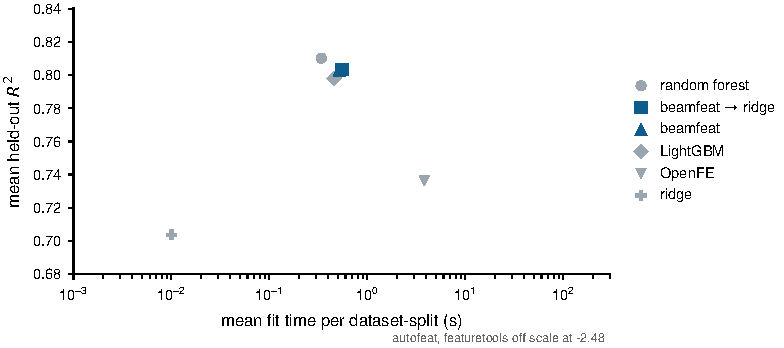
\includegraphics[width=0.85\linewidth]{figures/fig_accuracy_vs_cost.pdf}
\caption{Mean held-out $R^2$ against mean fit time across the 360-fit study,
on a logarithmic time axis. No error bars: the spread across the 45 fits per
method is dominated by differences between the nine datasets rather than by
uncertainty about a method, so an interval drawn from it would invite the wrong
reading. \texttt{featuretools} falls below the axis at $-2.48$.}
\end{figure}


\begin{figure}[tbp]
\centering
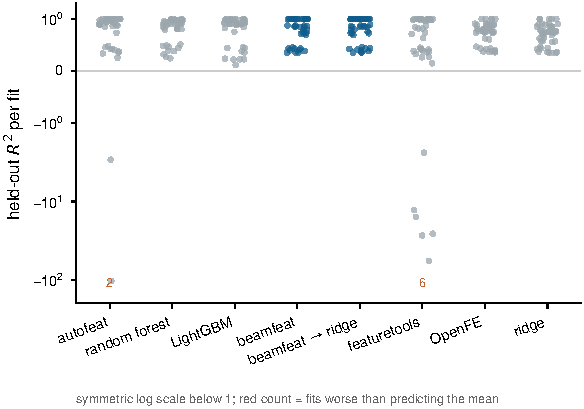
\includegraphics[width=0.78\linewidth]{figures/fig_fit_distribution.pdf}
\caption{Every fit in the comparison study, one column per method, on a
symmetric log scale below 1 so catastrophic results stay on the axis. A mean
conceals what the tail does: \texttt{featuretools} and \texttt{autofeat} each
produce fits far worse than predicting the target mean, while
\texttt{beamfeat}'s poorest result across all 45 fits is $R^2$ 0.355.}
\end{figure}

That study also records a reproducibility asymmetry: \texttt{beamfeat}
returns bit-identical results across runs given a seed: a determinism
test in the suite refits and compares formulas and predictions.
\texttt{autofeat} could not be made reproducible from outside. It exposes
no \texttt{random\_state}; its noise-injection feature screen draws
decoy features through the global NumPy generator, and the one seed it
sets internally (\texttt{np.random.seed(i)} per selection run) overrides
any seed a caller provides. Six runs
on one identical split of Friedman \#1, at the library's default
settings in the pinned environment, returned \(R^2\) from \(+0.952\) to
\(-109.8\) and between 17 and 26 selected features; pinning
\texttt{OMP\_NUM\_THREADS}, \texttt{NUMBA\_NUM\_THREADS} and
\texttt{MKL\_NUM\_THREADS} to 1 changed nothing. The variation appears
where selection is marginal, which is where it matters: on problems with
an unambiguous signal repeated processes agree exactly. It is visible at
the level of the whole study too: four executions of the nine-dataset
comparison returned \texttt{autofeat} mean \(R^2\) of 0.746, \(-1.69\),
0.754 and \(-1.56\), with worst single fits from \(-2.28\) to
\(-108.9\). Any single \texttt{autofeat} figure, including those above,
is one draw from that distribution. Catastrophic held-out scores are a
documented property of the method rather than an artifact of this
harness: Horn et al. \citep{horn2019} report test \(R^2\) of \(-12.4\)
on diabetes and \(0.048\) on Boston at three feature-engineering steps,
attributing it to tens of thousands of features fitted against fewer
than 500 rows. This study uses two steps, the library default, at which
their Table 2 reports no such failure. Further reproducibility signals:
370 automated tests including scikit-learn's own
\texttt{check\_estimator} compatibility suite; tests that exercise 95\%
of the code; automatic re-testing of every change (continuous
integration) against both the oldest supported and the newest dependency
versions; tutorial notebooks that execute end to end; and every figure
above produced by a script shipped in the repository.

The version described here is archived on Zenodo \citep{beamfeat}; the
development repository is at \url{https://github.com/LD-Shell/beamFeat},
and the package installs from PyPI as \texttt{pip\ install\ beamfeat}.

\hypertarget{discussion}{%
\section{Discussion and limitations}\label{discussion}}

Three limits bound what the measurements above establish. The marginal null
cannot see a feature that is jointly essential yet nearly independent of the
target on its own; Friedman \#1 prices that at roughly 0.086 of $R^2$, and
methods that select jointly do better on such structure while certifying
nothing. The comparison study spans nine datasets, which leaves the omnibus
test underpowered: it separates no pair of methods, and the paired tests carry
the inference. And every compared tool is run at default or paper-recommended
settings with no hyperparameter search, a protocol that understates
\texttt{OpenFE} in the gradient-boosted setting it was designed for and
\texttt{featuretools} outside its relational use case.

Two directions follow. Set-level scoring would close part of the remaining
search gap, but only by reintroducing the adaptivity the guarantee excludes;
whether a selective-inference correction can recover that power without
forfeiting error control is open. Second, the guarantee currently certifies
association rather than predictive contribution, and the post-fit holdout check
that separates them is a diagnostic, not a second guarantee.

\hypertarget{acknowledgements}{%
\section{Acknowledgements}\label{acknowledgements}}

The design of \texttt{beamfeat} was informed by a review of the
\texttt{autofeat} source code \citep{horn2019}, whose approach it builds
on and departs from as described above. The author conceived the method,
set its requirements and acceptance criteria, and directed development, using Anthropic's Claude as an AI assistant for implementation and drafting. Every figure and table in
this paper is regenerated by a script that ships in the repository, and
the full tests run automatically on every change. The one exception is
noted where it arises: three of the four executions of the comparison
study were superseded and their per-fit records not retained, so those
means are reported from run transcripts rather than archived data. The
author reviewed all code and text and takes sole responsibility for the
work. This work received no external funding.

\renewcommand\refname{References}
  \bibliography{paper}

\end{document}